\section{Muon Decay at \mueee}
\mueee \cite{Blondel:2013ia} is a proposed experiment, currently under construction, that will look for the decay of $\mu^+ \rightarrow e^+ e^+ e^-$, which violates lepton flavour.
This experiment will operate at the Paul Scherrer Institute (PSI) in Switzerland, and is currently taking data in its first phase for 2015-2016.
A second phase for 2017 and beyond is planned, and the details of the phases are covered in this section. 
Lepton flavour violating (LFV) decays are allowed within the SM once one includes the neutrino masses.
Since we see LFV processes in the nuetrino sector, due to nuetrino mixing, it is not unreasonable to expect that there may also be new physics that violates lepton number in the charged lepton sector.
\mueee is aiming to find BSM LFV by investigating such $\mu^+$ decays.
The SM process for $\mu^+ \rightarrow e^+ e^+ e^-$ is show in Fig. \ref{fig:mu_eee_SM}.
\begin{figure}[h]
    \centering
    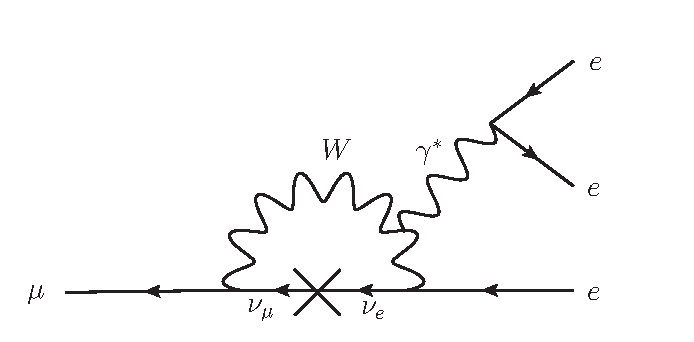
\includegraphics[height = 1.5in]{Figures/feynman_diagrams/mu_eee_SM.eps}
    \caption[$\mu^+ \rightarrow e^+ e^+ e^-$ lepton flavour violating decay through neutrino oscillation.]{$\mu^+ \rightarrow e^+ e^+ e^-$ LFV decay with a muon neutrino oscillating to an electron neutrino. This process is heavily suppressed due to the neutrino oscillation required.}
    \label{fig:mu_eee_SM}
\end{figure}
For this process, the required neutrino oscillation which mediates the lepton flavour violating component suppresses the branching ratio of this process, so much so that $\textrm{BR}(\mu^+ \rightarrow e^+ e^+ e^-) \ll 10^{-50}$.
This is an unobservably low decay rate, and so any decays of this form will almost certainly be a sign for new physics.

New physics may come in the form of new particles that can mediate these loops without a penalty like the neutrino mixing, if it is to be observed.
This could be in the form of supersymmetric particles in a loop, or other particles which add couplings to muons and electrons.
It is also possible that a new mediator adds observable contributions at tree level.

The current experimental limits on the branching ratio of various muon decay processes is shown in Table \ref{table:mu_br_limits}.

\begin{table}[h]
\label{table:mu_br_limits}
\begin{center}
\begin{tabular}{|l|l|l|} \hline
Decay Channel & Experiment & Branching Ratio \\ \hline
$\mu \rightarrow e \gamma$ & \mega & $< 1.2\times 10^{-11}$ \\
& \meg & $< 2.4\cdot 10^{-12}$ \\ \hline
$\mu \rightarrow eee$ & \sindrum & $< 1.0\times 10^{-12}$ \\ \hline
$\mu~Au\rightarrow e~Au$ & \sindrumii & $< 7\times 10^{-13}$ \\ \hline
\end{tabular}
\end{center}
\caption{Branching ratio limits on muon decay from various experiments as given in \cite{Blondel:2013ia}.}
\end{table}

Note that all of these upper limits are on the order of $10^{-10} - 10^{-13}$.
Any future experiments must examining these decay modes must be sensitive to branching ratios at least as small as the upper limits here.
For this reason, \mueee is attempting to reach branching ratios down to $10^{-16}$ for the $\mu \rightarrow eee$ process.
To reach such a low branching ratio, at least $5.5 \times 10^{16}$ muon decays must be observed, if one assumes a total efficiency of $30\%$.

Given that this many muon decays are possible, the muon beam will be placed onto a aluminium target to stop the muons.
The decay products of the muons are then tracked with the detector.
A schematic of the target with the muon beam in shown in Fig. \ref{fig:mu3e_target}.

\begin{figure}[h]
    \centering
    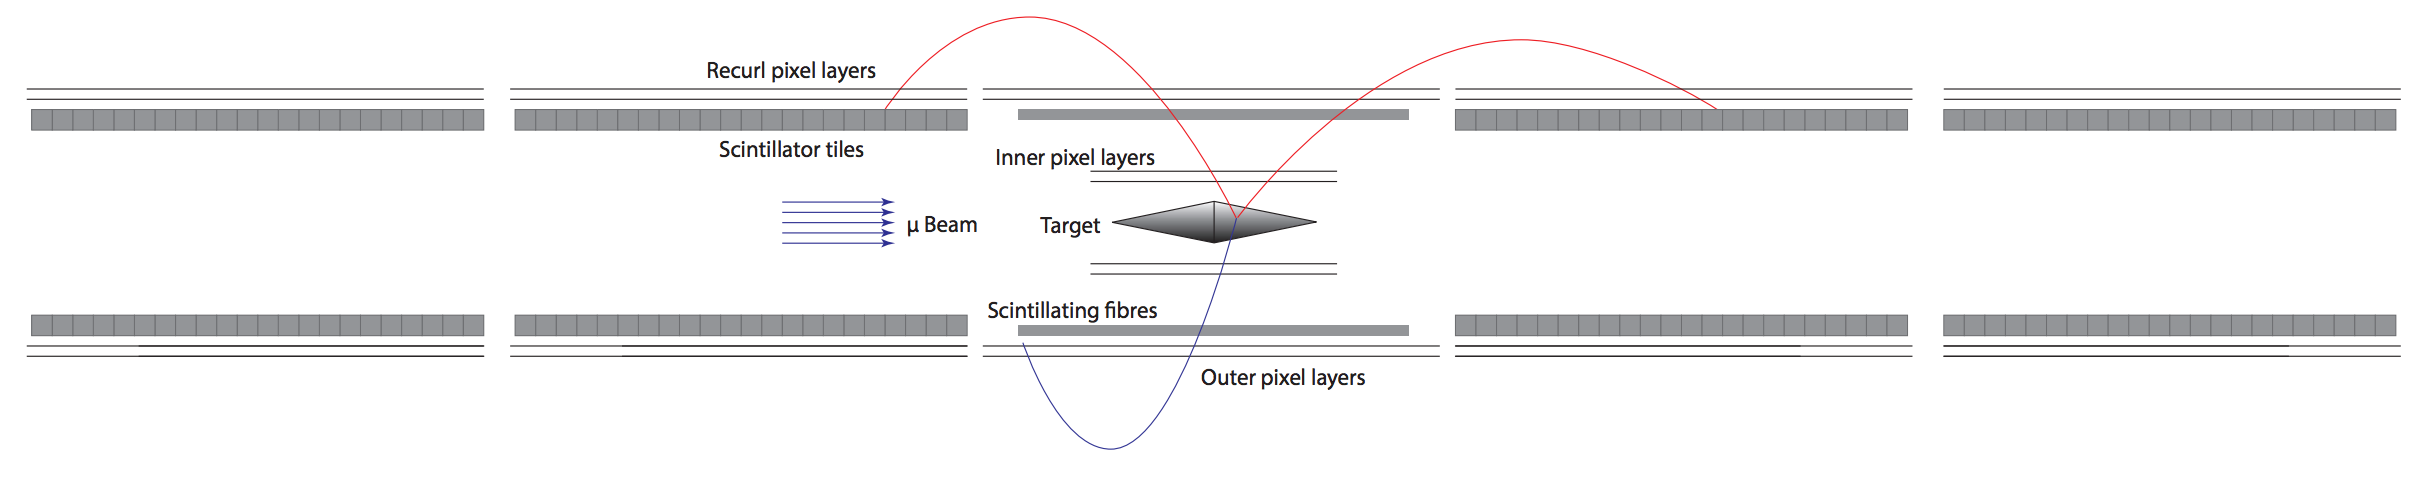
\includegraphics[width = \textwidth]{Figures/experiments/mu3e_target.png}
    \caption{Schematic of a muon decay in the full \mueee detector \cite{Blondel:2013ia}.}
    \label{fig:mu3e_target}
\end{figure}

In order to achieve such a low sensitivity, and for practical purposes of building and commissioning the detector, \mueee plans to run in two distinct phases of operation.
The differences between these two phases lies primarily in the differences between the beam lines, which will be discussed below.
However, there are also planned additions/modifications to the detector.

\subsection{Phase I}
The first phase will aim for a branching ratio sensitivity of $10^{-15}$.
PSI currently produces muons at a rate that \mueee can take advantage of for the first phase, without modifications, and can additionally serve as a commissioning time.
To produce the muons used, phase I will use the existing $\pi\textrm{E5}$ beam line.
This is done by colliding protons on target to produce pions, proceeding by the strong interaction in equation \ref{eqn:pion_production}.

\begin{equation}
\label{eqn:pion_production}
p^+ + p^+ \rightarrow p^+ + n + \pi^+
\end{equation}

\noindent Note that this is process is independent of the target $Z$, since the interaction takes place direclty between the proton beam and a single proton on target.
However, a carbon target is chosen due to, among other reasons, good heat disappation and the high density allows for a compact target with good pion production per unit volume of target.
For production to be possible, the excess centre of mass energy must be at least as large as the pion mass, giving a threshold energy of $290\textrm{MeV}$ for the proton beam.
To get a reasonable yield of pions, a $590\textrm{MeV}$ proton beam is used, producing low energy ($10-120\textrm{MeV}$) pions.
A beam current of $2.3\textrm{mA}$ will be used.

Pions that have stopped near the surface of the target, give rise to surface muons, where the pion decays through the weak force to muons as shown in equation \ref{eqn:muon_production}.

\begin{equation}
\label{eqn:muon_production}
\pi^+ \rightarrow \mu^+ + \nu_\mu
\end{equation}

\noindent The pions have incredibly short lifetimes, $2.6 \times 10^{-8}s$, and the branching ratio of this process is very large, $\textrm{BR}(\pi^+ \rightarrow \mu^+ + \nu_\mu) = 99.98770\%$ \cite{Agashe:2014kda}.
One does not have to wait long then to have a good source of surface muons.
An expected number of $10^{15}$ muon decays can be expected during this phase.
Since the pions decaying are at rest, and the muon has a mass very close to that of the pion, the muons are produced with momenta of $28\textrm{MeV}$.
These are easy collimate and provide a very monochromatic beam of muons, since only $10\%$ of the surface muons can be used from an angular selection.
The collimated beam of positively charged muons is then directed to a target within a solenoidal magnetic field at a rate of $2 \times 10^8 \mu^+/s$.
A schematic of the beam line that produces the muon beam is shown in Fig. \ref{fig:mueee_phaseI_schematic}.

\begin{figure}[h]
    \centering
    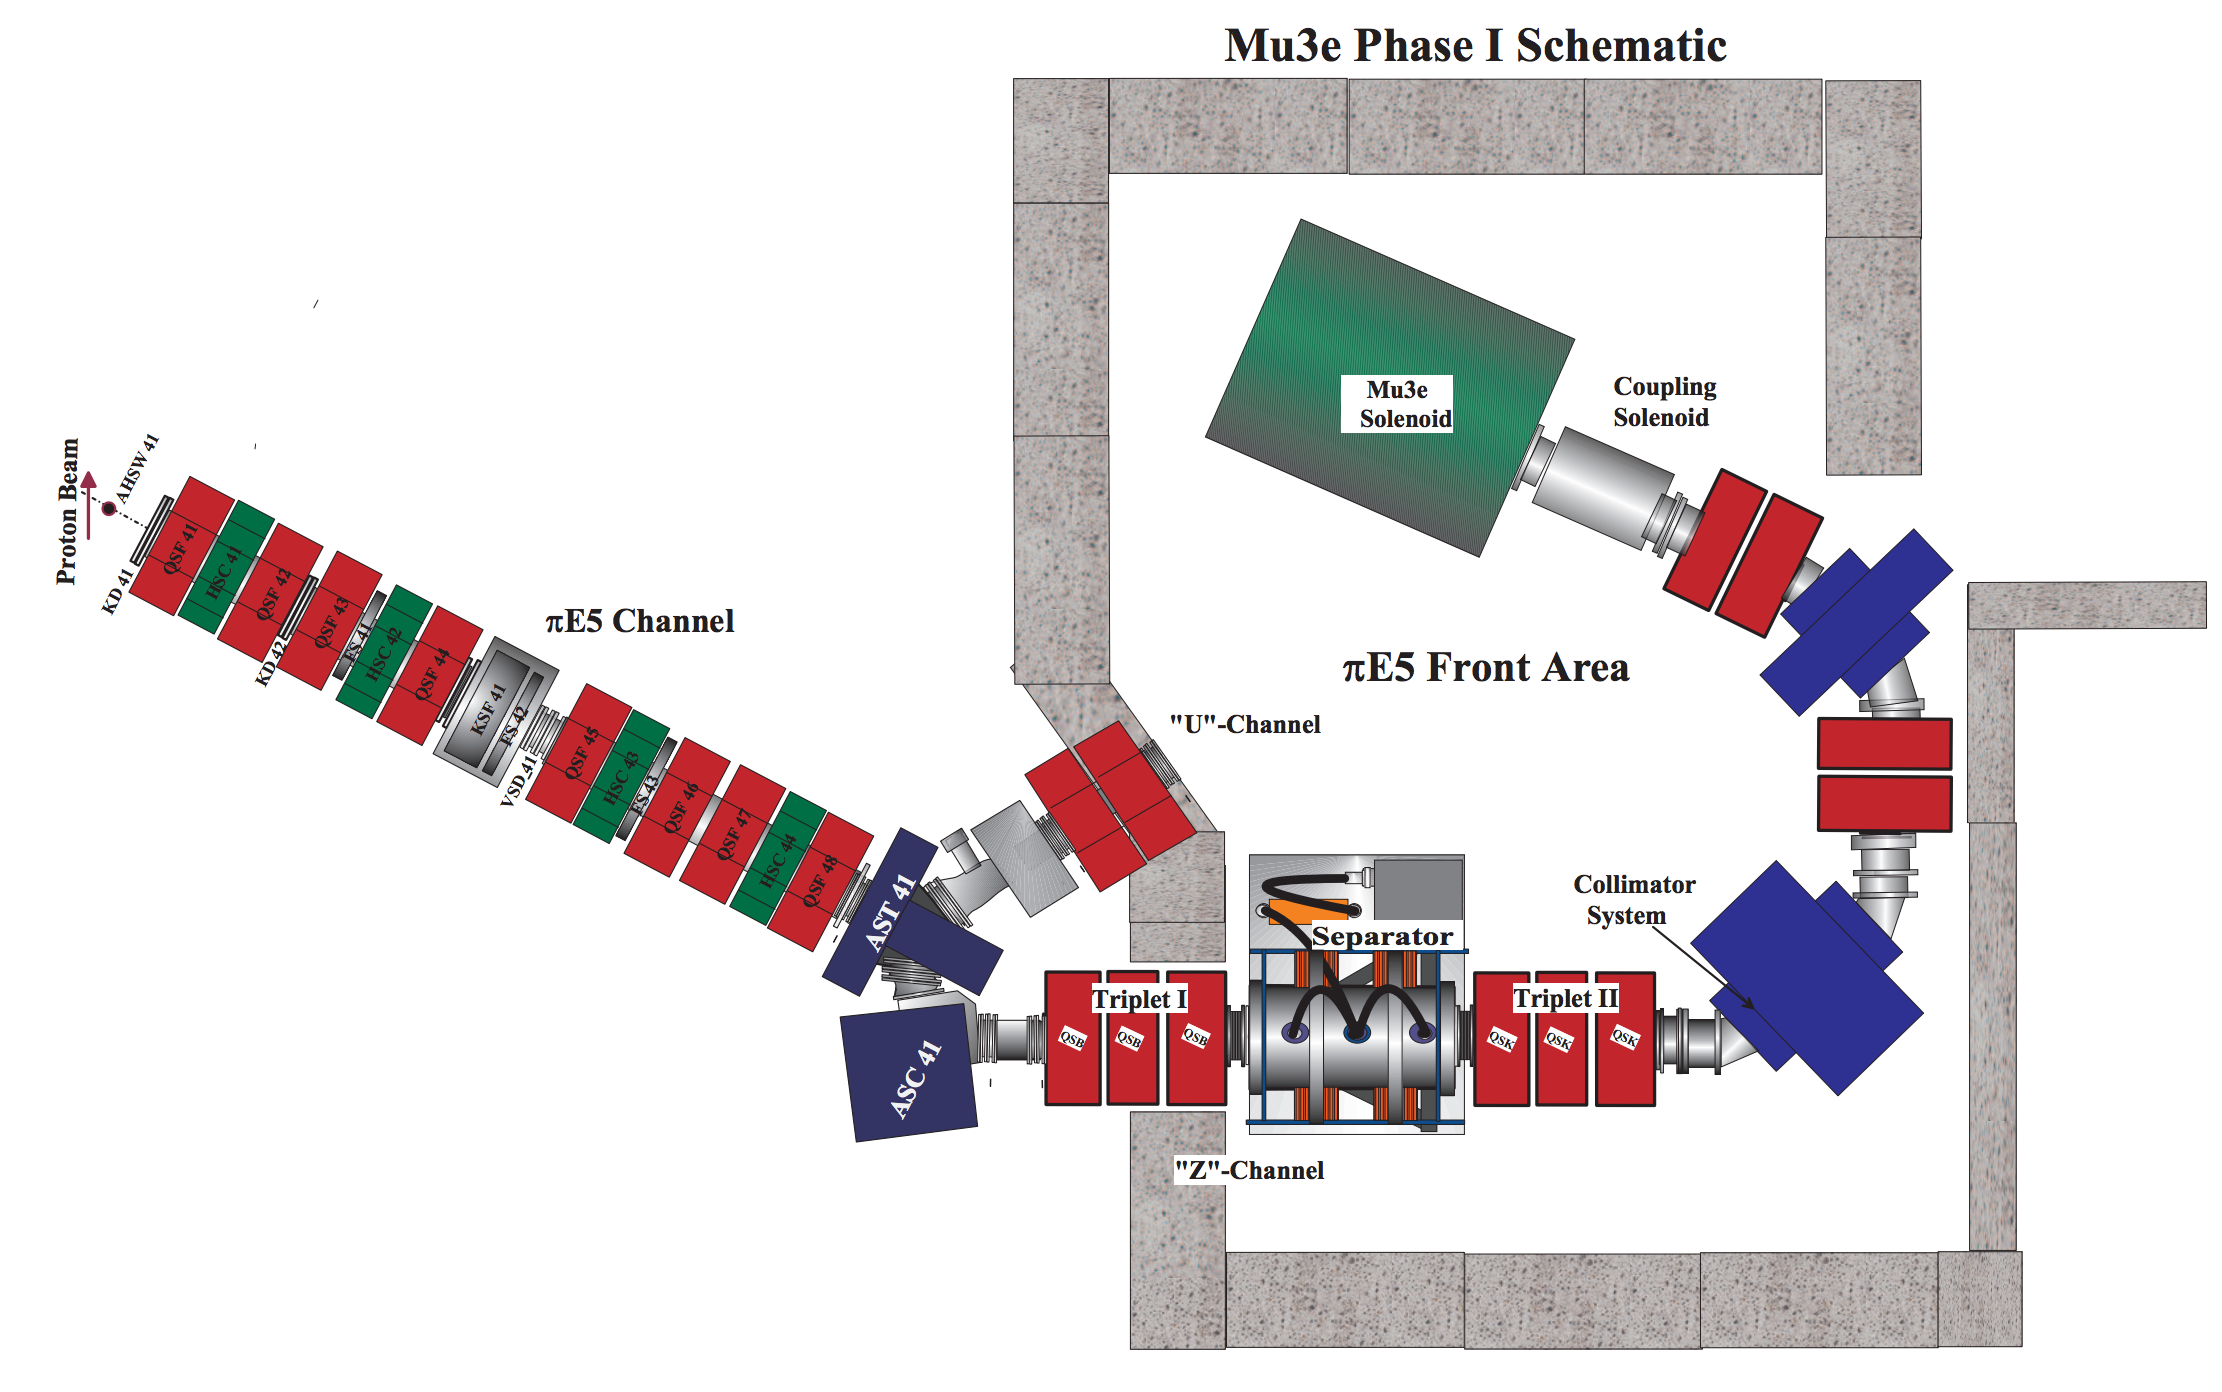
\includegraphics[width = \textwidth]{Figures/experiments/mu3e_phase1_schematic.png}
    \caption{\mueee phase I beam line schematic using the $\pi\textrm{E5}$ at PSI, from \cite{Blondel:2013ia}.}
    \label{fig:mueee_phaseI_schematic}
\end{figure}

During this time, the detector is relatively minimal compared to the full run planned, and curently is using a pixel-only detector.
The target is surrounded with a set of inner and outer silicon pixel detectors, allowing the determination of momentum, vertex position, and decay time.
Phase I is actually split into phase IA and phase IB, where a detector upgrade will occur in phase IB.
The silicon pixel detectors in phase IA have relatively poor precision in momentum and timing, and are the target of the upgrades.
Even so, phase IA will have sensitivity on the branching ratios down to $\order(10^{-14})$.

For phase IB, the first pair of recurl pixel layers will be added, along with the tile detectors and the fibre tracker.
The recurl stations allow for the decay products to be seen as coming in from outside the detector, as the radius the charged decay products will take is typically larger than the detector.
Improvements from adding the recurl stations with the tile detectors allows for momentum resolution of $0.44\textrm{MeV}$.
Similarly, the fibre tracker and tile detector also improve the timing resolution to $\order(100-300\textrm{ps})$. 
Also worth noting is the total energy resolution, which is less than $1\textrm{MeV}$.
